\documentclass[11pt,a4paper]{article}
\usepackage{fontspec}
\setmainfont{TeX Gyre Pagella}
\newfontfamily\headfont{Inter}[UprightFont=*-ExtraBold,BoldFont=*-ExtraBold,Extension=.otf,Path=/usr/share/fonts/opentype/inter/]
\usepackage[a4paper,margin=2.3cm]{geometry}
\usepackage{graphicx,booktabs,float,caption,array,xcolor,longtable}
\usepackage{xurl}
\usepackage[hidelinks]{hyperref}
\usepackage{titlesec}
\usepackage[round]{natbib}
\usepackage{setspace}
\setstretch{1.05}
\renewcommand{\topfraction}{0.9}
\renewcommand{\bottomfraction}{0.8}
\renewcommand{\textfraction}{0.1}
\renewcommand{\floatpagefraction}{0.75}
\setlength{\parindent}{0pt}
\setlength{\parskip}{0.55em}
\titleformat{\section}{\headfont\Large}{\thesection}{0.8em}{}
\titleformat{\subsection}{\headfont\large}{\thesubsection}{0.8em}{}
\captionsetup{font=small,labelfont=bf}
\urlstyle{same}
\hypersetup{pdftitle={How Accurate Were Portolan Charts?},pdfauthor={Tristan Hotham}}

\begin{document}
\begin{center}
{\Large\bfseries How Accurate Were Portolan Charts?\par}
\vspace{0.4em}
{\large The Carta Pisana and the Catalan Atlas measured against the real coast\par}
\vspace{1.2em}
{\large Tristan Hotham\par}
\vspace{0.3em}
{\small Independent researcher\\
ORCID: 0000-0003-4931-9349\\
DOI: https://doi.org/10.5281/zenodo.24044645\par}
\vspace{0.8em}
2026
\end{center}

\begin{quote}
\small
\begin{center}\textbf{Abstract}\end{center}
Portolan charts, the compass-line sea charts of the Mediterranean that appear in the late thirteenth century, are famous for an accuracy that no other map of their time approaches. I measure it on the two best-known early examples from public domain scans: the Carta Pisana (about 1275) and the chart of the Catalan Atlas (1375). I read 148 and 100 coastal control points by eye (harbours, headlands, river mouths and islands; for the faded Pisana with the help of Jomard's facsimile, carried back to the original by a thin-plate spline through the compass-line nodes), identified each and fitted the true positions to the chart positions. A single scale and rotation leaves a median error of 93 km on the Pisana and 119 km on the Catalan Atlas. Both charts are rotated anticlockwise against true north, by 10.4 and 11.2 degrees; directions between pairs of places are a median 10.2 degrees off as drawn and 2.1 degrees off (Pisana) once that rotation is removed. Locally the charts are better still: judged from its eight nearest neighbours the median Pisana place is 38 km out. Fitted basin by basin, the western and eastern Mediterranean of the Pisana have median errors of 36 and 43 km, while its Atlantic coasts are 312 km out under the whole-chart fit and drawn 18\% too small. The Catalan Atlas repeats the pattern a century later. An equirectangular frame fits both charts at least as well as Mercator. Measured the same way, Ptolemy's Geography misses by a median 144 km and the Hereford Mappa Mundi by 516 km.

\textbf{Keywords:} portolan charts; Carta Pisana; Catalan Atlas; cartometry; map accuracy; magnetic declination; history of cartography
\end{quote}

\section{Introduction}
The portolan chart is the great puzzle of medieval cartography. The oldest to survive, the Carta Pisana, is usually dated to the last decades of the thirteenth century; within a hundred years the type was being drawn in Genoa, Venice, Majorca and Barcelona with a stable outline of the Mediterranean and the Black Sea that is startlingly close to the real one \citep{campbell1987}. The charts carry no graticule. They are built on networks of compass lines radiating from one or two circles of sixteen points, with the names of harbours written inland at right angles to the coast. How they were made, and whether their accuracy implies a lost survey or projection, has been argued for a century \citep{lanman1987,nicolai2016}.

This paper does not try to settle how they were made. It asks a narrower question with open data and a reproducible method: how accurate are the two most famous early charts, where are they good and where are they bad, and how do they compare with the other medieval and ancient world pictures I have measured the same way \citep{hotham_ptolemy,hotham_hereford,hotham_idrisi}? Section~\ref{sec:data} describes the scans and the readings, Section~\ref{sec:methods} the fits, Section~\ref{sec:results} the results and Section~\ref{sec:limits} what they cannot show.

\section{Data}\label{sec:data}
\subsection{The charts}
The Carta Pisana is held by the Biblioth\`eque nationale de France (Cartes et plans GE B-1118); I use the public domain scan on Wikimedia Commons (3,481 by 1,848 pixels). Its ink is badly faded, especially in the east, and the eastern Black Sea is largely lost. To read the names I also used the lithographed facsimile by Jomard in \textit{Les monuments de la g\'eographie} \citep{jomard}, but every position used in the analysis is a position on the original scan (Section~\ref{sec:transfer}).

The Catalan Atlas (BnF Espagnol 30) is a set of panels on vellum; the chart occupies panels 5 to 8 from west to east, with north at the top, and panels 1 to 4 hold the cosmographical text and calendar. I use the per-panel Commons scans at half size (about 3,230 by 7,900 pixels each). The atlas is usually attributed to the workshop of Cresques Abraham in Majorca.

\subsection{Readings}
No open table of control points exists for either chart: the published toponymic tables give the order and presence of names, not positions \citep{campbell1987,pujades2007}. I therefore read points by eye on zoomed crops with a pixel grid: harbours where the name or town sign makes the point clear, headlands and river mouths read from the drawn coast, and island centres or tips. Each reading has my identification, its modern latitude and longitude and a confidence flag (1: clear name and certain place; 2: probable; 3: the place is certain but the exact point, or the reading of the name, is doubtful). The typed positions were checked against the Natural Earth 1:10 million coastline: the median distance from the coast is 0.7 km, and every point more than 15 km inland or offshore is an island centre, an estuary or an islet too small for that coastline.

There are 148 Pisana readings (77 western Mediterranean, 51 eastern Mediterranean, 3 Black Sea and 17 Atlantic) and 100 Catalan Atlas readings (38, 29, 6 and 27). On the Pisana 42\% of readings have confidence 1 or 2. The Mediterranean is split at 16 degrees east (Cape Bon, Sicily and the Strait of Messina), with the whole Adriatic in the east; the Atlantic includes the Biscay, Channel and North Sea coasts, Britain, Ireland, Morocco beyond Gibraltar and the Atlantic islands.

\subsection{From the facsimile to the original}\label{sec:transfer}
93 of the Pisana readings were made on Jomard's facsimile. The facsimile is a careful tracing but not a geometric copy, so its positions are carried to the scan by a smoothed thin-plate spline through 24 nodes of the two compass circles (found automatically on the facsimile as points where many straight lines meet, and read by eye on the scan) and the 12 places read on both images with confidence 1 or 2. Leaving each of those places out in turn, the spline predicts its position on the scan to a median 23.8 pixels (about 37 km at the chart's scale; maximum 37.0 pixels). Where a place was read on both images (19 places) the reading on the scan is used. Figure~\ref{fig:reading} shows the two images side by side.

\begin{figure}[tbp]\centering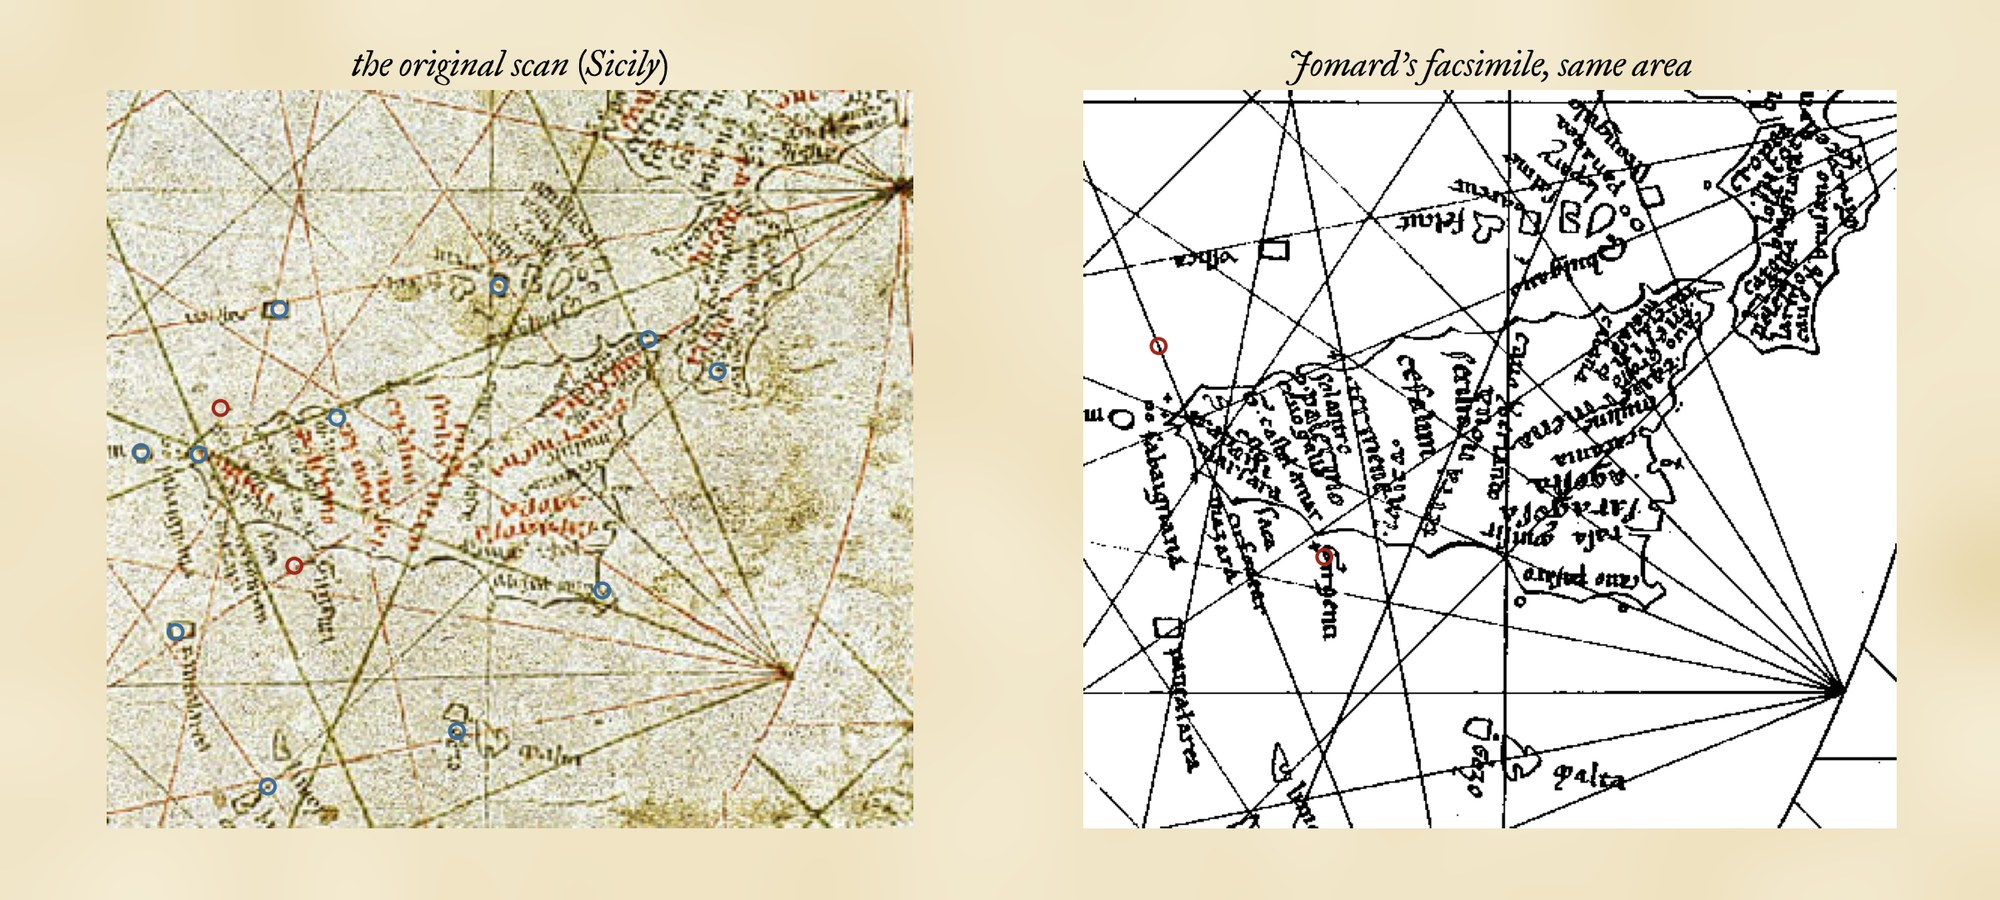
\includegraphics[width=\textwidth]{f_reading.jpg}
\caption{Reading the Pisana. Left: the original scan around Sicily, with places read directly (blue) and carried from the facsimile (red). Right: the same area on Jomard's facsimile.}\label{fig:reading}\end{figure}

\subsection{Joining the Catalan panels}
The four chart panels were placed side by side, each cropped to its own vellum. The folds hide part of the drawing, so the panels cannot simply be abutted: a compass rose cut by the fold between panels 6 and 7 has its centre 102 pixels apart on the abutted mosaic, and I shift panels 7 and 8 by that amount. No such mark crosses the other two folds. As a sensitivity test, a free offset for every panel (two extra parameters each) reduces the median error only to 108 km, and the fitted offsets are implausibly large, because they absorb real distortion.

\section{Methods}\label{sec:methods}
Chart positions $z$ (pixels, with $y$ turned upward) are related to projected true positions $w$ by a similarity transformation $z = aw + t$ ($a$ and $t$ complex: one scale, one rotation and a shift, four parameters) or a general affine one (six). The projections are Mercator, the equirectangular projection with standard parallel 38\textdegree{} N, and an azimuthal equidistant projection about the centroid of the points. Errors are measured on the globe: each chart point is carried back through the inverse fit and projection, and the error is the great-circle distance to the true place. The rotation of the similarity fit is the chart's tilt: positive values mean the chart is turned anticlockwise against true north.

\textbf{Basins.} Each basin with at least eight points is also fitted on its own, giving its own rotation, its scale relative to the whole chart, and its own median error. \textbf{Local error.} Each place is predicted from an affine fit (on Mercator) to its eight nearest neighbours by true distance, as in my study of al-Idrisi's map \citep{hotham_idrisi}; this measures how well a place agrees with its surroundings, independent of how the basins are joined. \textbf{Directions.} For every pair of places at least 100 km apart I compare the direction on the chart with the true rhumb-line (Mercator) bearing, as drawn and after turning the chart back by its fitted rotation. \textbf{Distortion grid.} A smoothed thin-plate spline from Mercator to the chart carries the 5\textdegree{} graticule and the Natural Earth coast onto each chart; it is drawn only within about 400 km of a control point and only in basins with at least five points.

\section{Results}\label{sec:results}
\subsection{The whole chart and the tilt}
The best similarity fit on Mercator leaves a median error of 93 km on the Pisana (90th percentile 191 km) and 119 km on the Catalan Atlas (302 km); an affine fit improves these to 92 and 96 km. Both fits need a rotation: 10.4 degrees anticlockwise for the Pisana and 11.2 for the Catalan Atlas (Figure~\ref{fig:charts}). The same tilt appears in the directions between places (Figure~\ref{fig:bearings}): over 10,738 Pisana pairs the median signed error is -10.1 degrees, and 94\% of pairs are turned anticlockwise; over 4,914 Catalan pairs, -10.2 degrees and 96\%. Turned back, the median absolute error is 2.1 degrees on the Pisana, with 78\% of pairs within 5 degrees, and 3.6 degrees on the Catalan Atlas (62\%).

The rotation is commonly attributed to magnetic declination, the charts having been compiled from compass courses \citep{campbell1987,lanman1987}. The measurement cannot test that directly, but it shows that the tilt is about the same on two charts made a century apart, and on the Pisana nearly identical in the western and eastern basins fitted separately (9.7 and 10.0 degrees).

\begin{figure}[tbp]\centering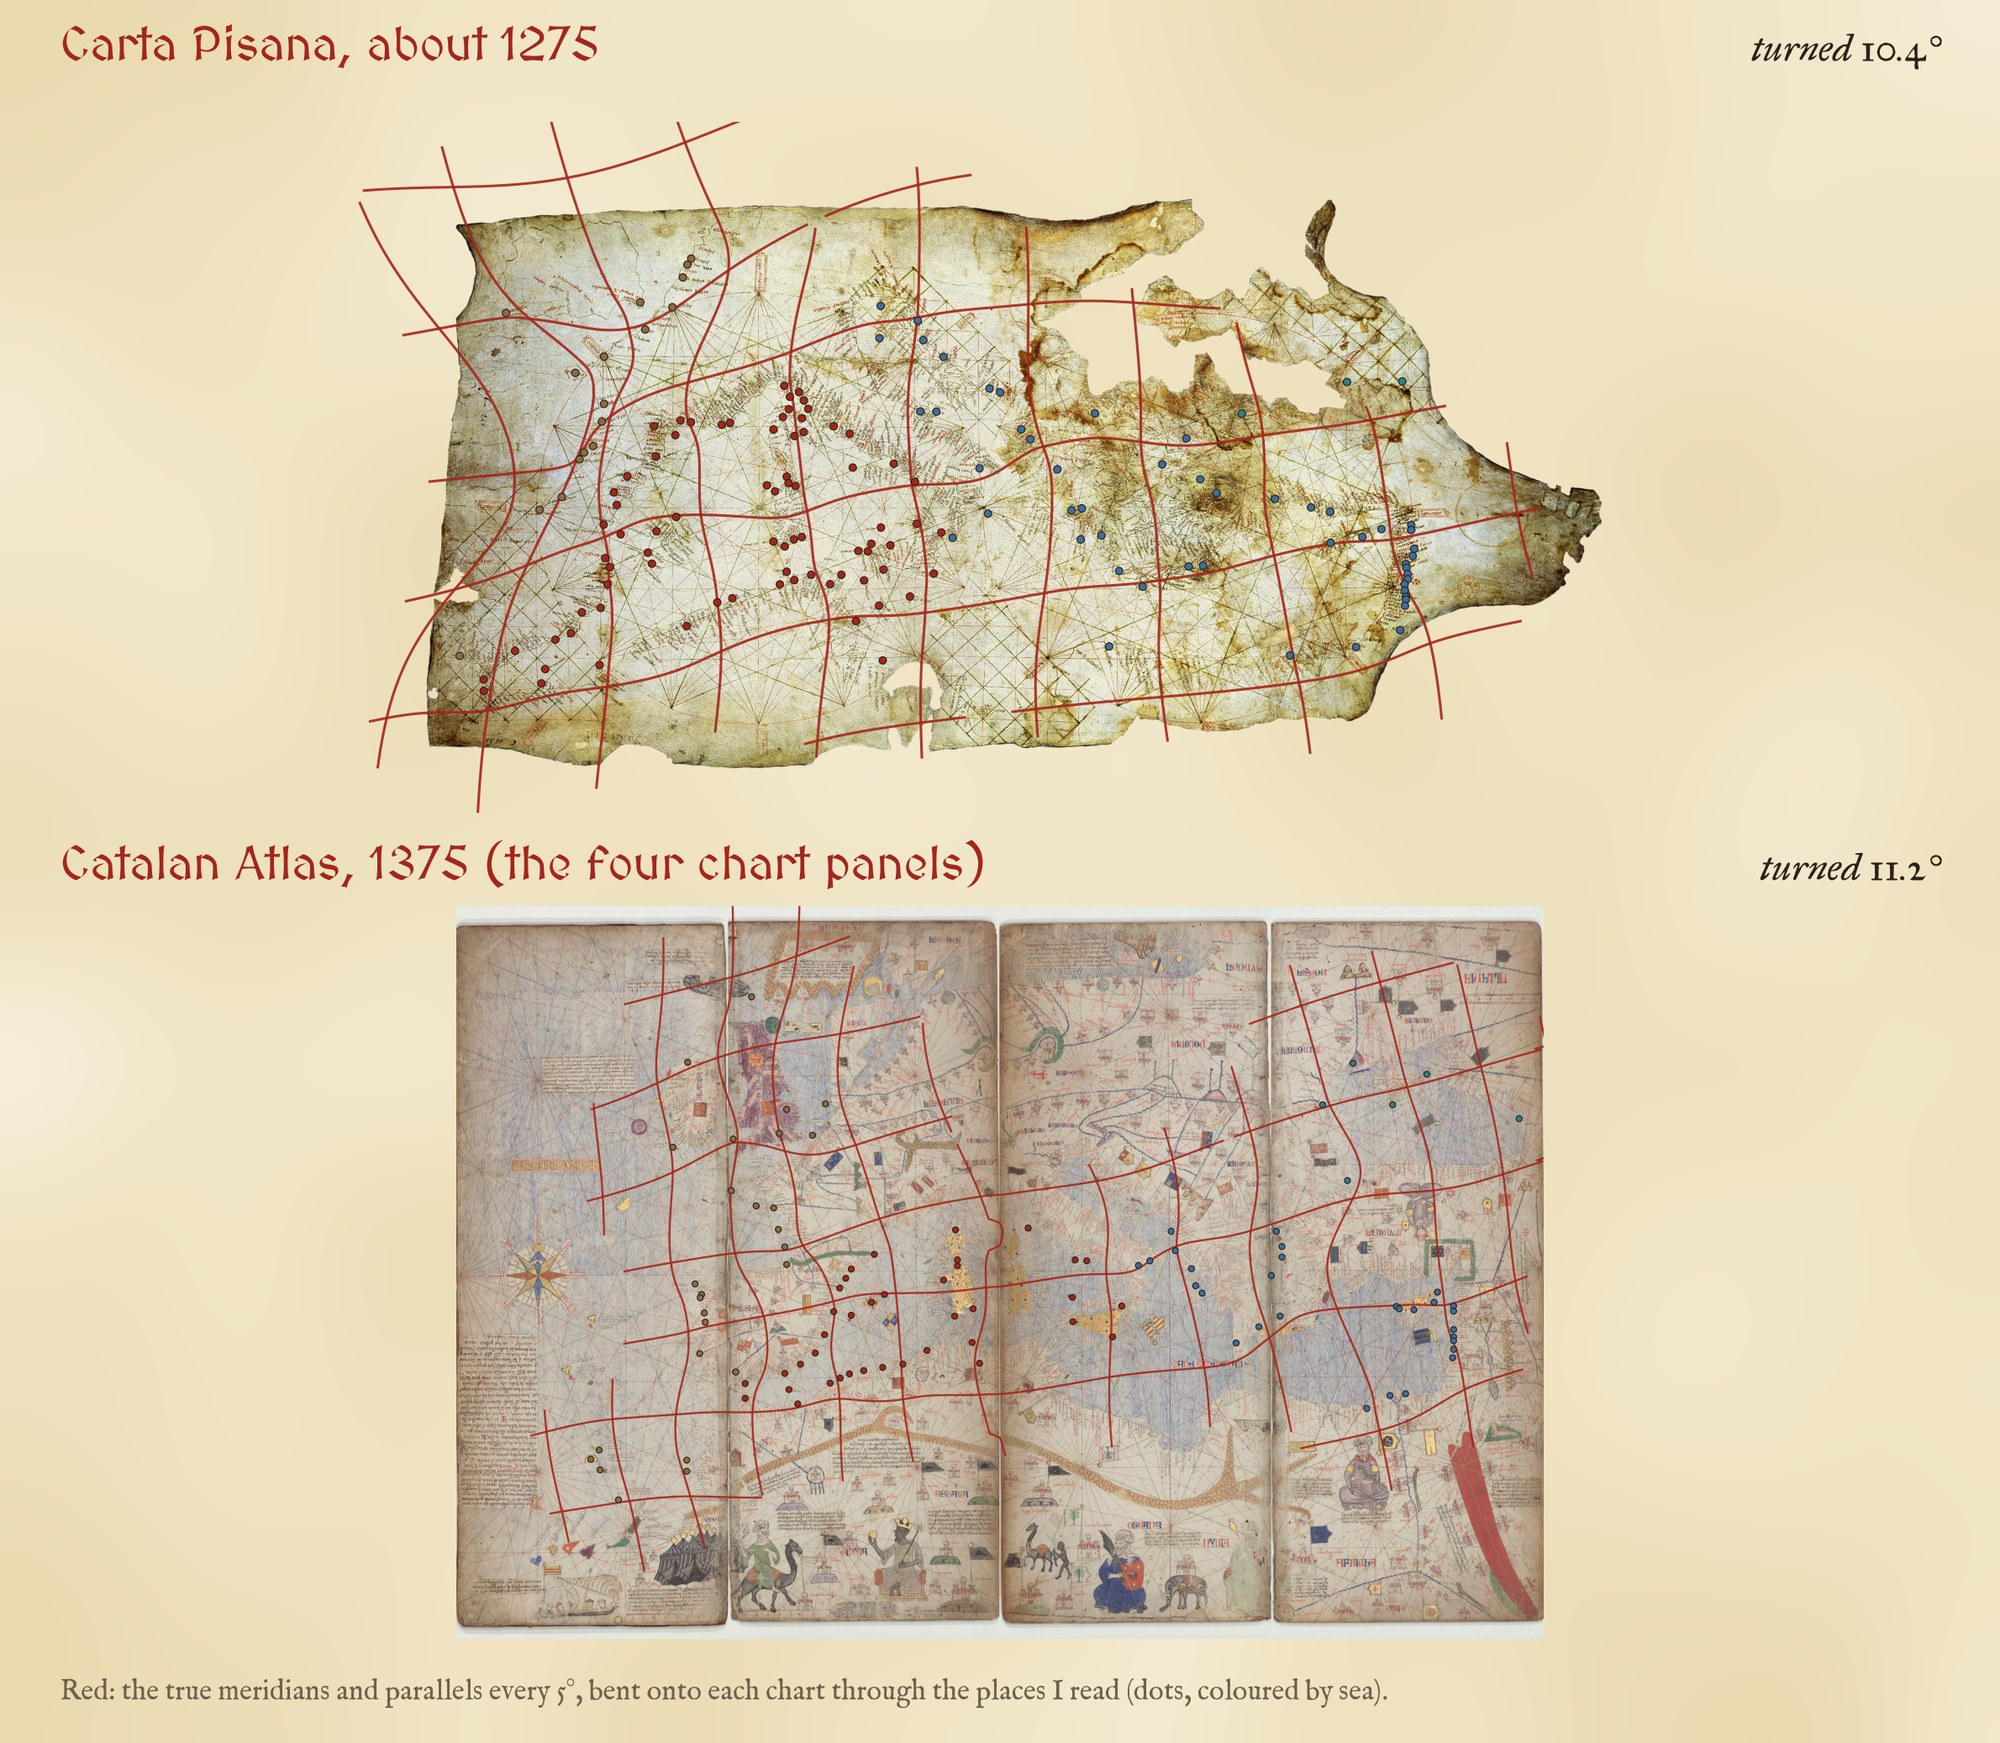
\includegraphics[width=\textwidth]{f_charts.jpg}
\caption{The two charts with the true 5\textdegree{} graticule carried onto them by a thin-plate spline through the control points (dots, coloured by basin as in Figure~\ref{fig:basins}).}\label{fig:charts}\end{figure}

\begin{figure}[tbp]\centering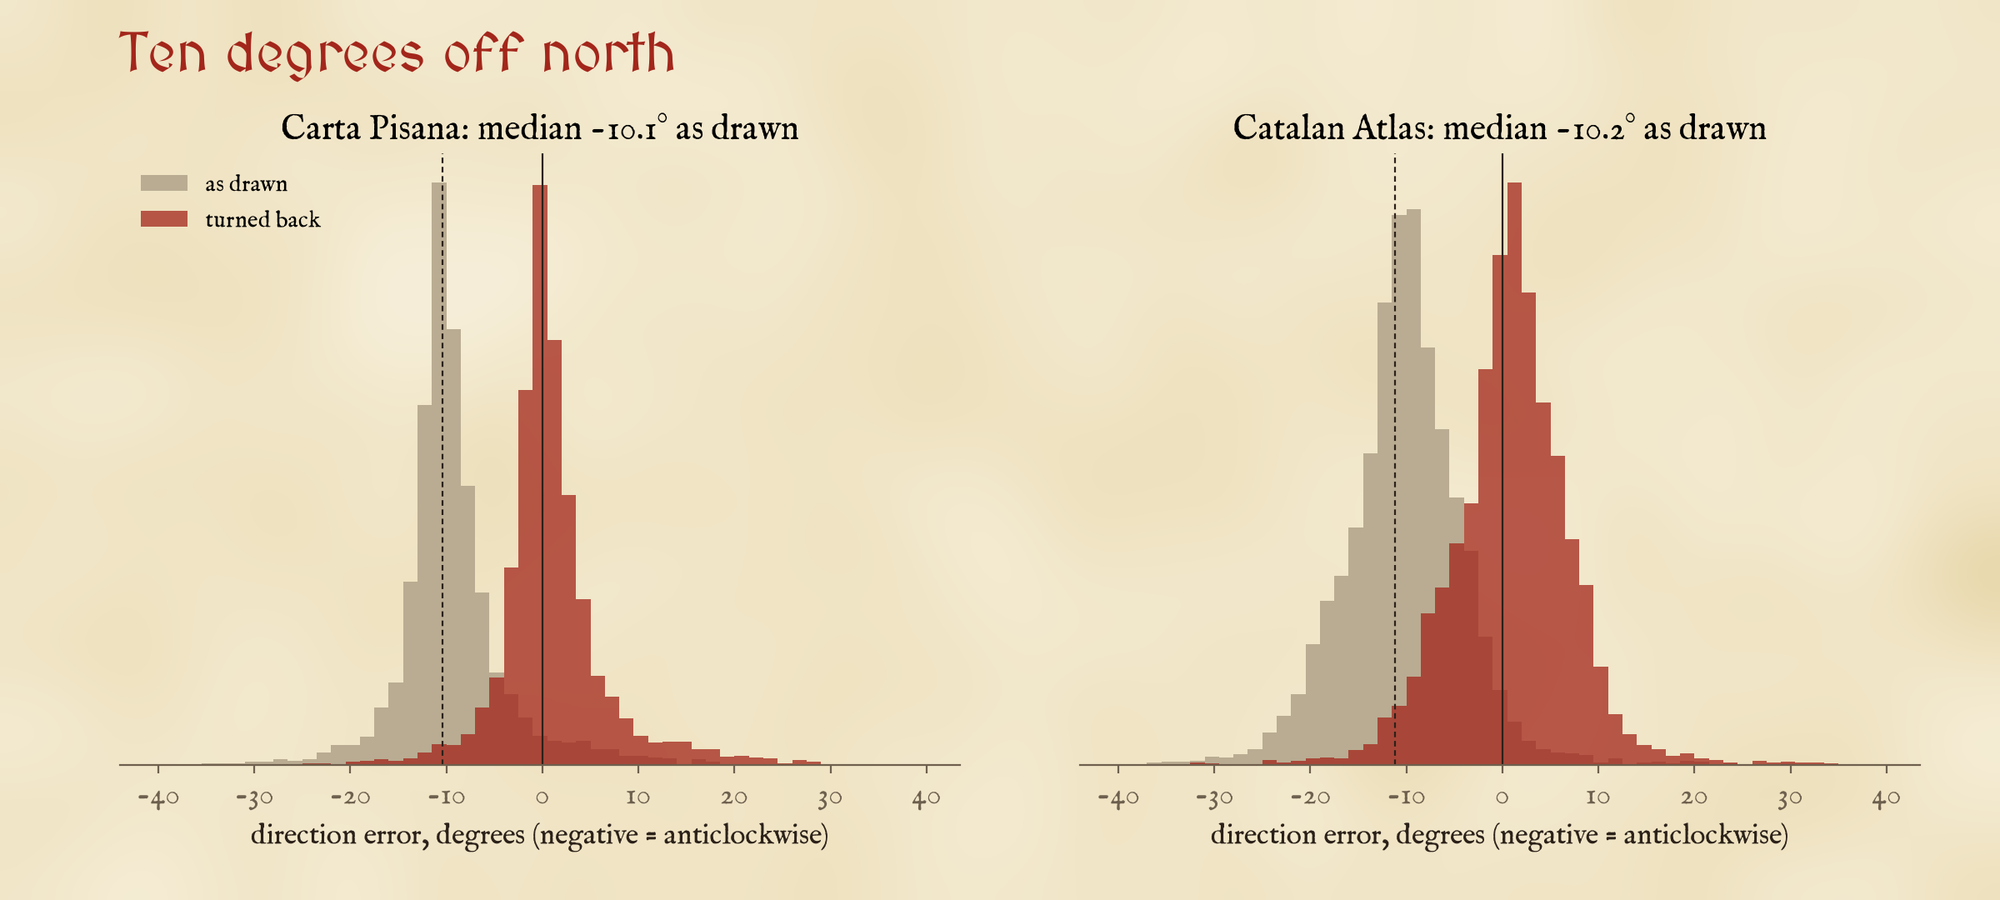
\includegraphics[width=\textwidth]{f_bearings.png}
\caption{Direction on the chart minus the true rhumb-line direction, for every pair of places at least 100 km apart. Grey: as drawn. Red: after removing the fitted rotation. The dashed line marks the fitted rotation.}\label{fig:bearings}\end{figure}

\subsection{Basin by basin}
Table~\ref{tab:basins} and Figure~\ref{fig:basins} give the errors by basin. Under the whole-chart fit, the Pisana's Mediterranean places are a median 86 km (west) and 81 km (east) out, and its Atlantic places 312 km, 3.7 times as far. Fitted on their own, the Mediterranean basins fall to 36 and 43 km and the Atlantic to 99 km, with a scale 0.82 times that of the whole chart. On the Catalan Atlas the Atlantic is 244 km out under the whole-chart fit and drawn at 0.76 of the chart's scale; its worst places are in Scotland and Ireland. Figure~\ref{fig:arrows} maps the residuals.

The local error is smaller still: a median 38 km on the Pisana (30 km in the west, 40 km in the east, 111 km on the Atlantic coasts) and 55 km on the Catalan Atlas. On the Pisana, places read directly on the scan have a median local error of 34 km, those carried from the facsimile 40 km: part of the local error is my transfer, not the chart.

\begin{table}[tbp]\centering\small\caption{Errors by basin (medians, km): under the whole-chart similarity fit, under the basin's own fit (with its rotation in degrees and its scale relative to the whole chart), and the local error from the eight nearest neighbours.}\label{tab:basins}\begin{tabular}{llrrrrrr}\toprule Chart & Basin & n & Whole & Own & Turn & Scale & Local\\\midrule
Carta Pisana & Western Mediterranean & 77 & 86 & 36 & 9.7 & 1.02 & 30\\
Carta Pisana & Eastern Mediterranean & 51 & 81 & 43 & 10.0 & 1.05 & 40\\
Carta Pisana & Black Sea & 3 & 117 &  &  &  & \\
Carta Pisana & Atlantic coasts & 17 & 312 & 99 & -2.1 & 0.82 & 111\\
Catalan Atlas & Western Mediterranean & 38 & 121 & 57 & 5.4 & 1.03 & 43\\
Catalan Atlas & Eastern Mediterranean & 29 & 83 & 56 & 12.6 & 1.04 & 61\\
Catalan Atlas & Black Sea & 6 & 111 &  &  &  & 42\\
Catalan Atlas & Atlantic coasts & 27 & 244 & 73 & 4.1 & 0.76 & 62\\
\bottomrule\end{tabular}\end{table}

\begin{figure}[tbp]\centering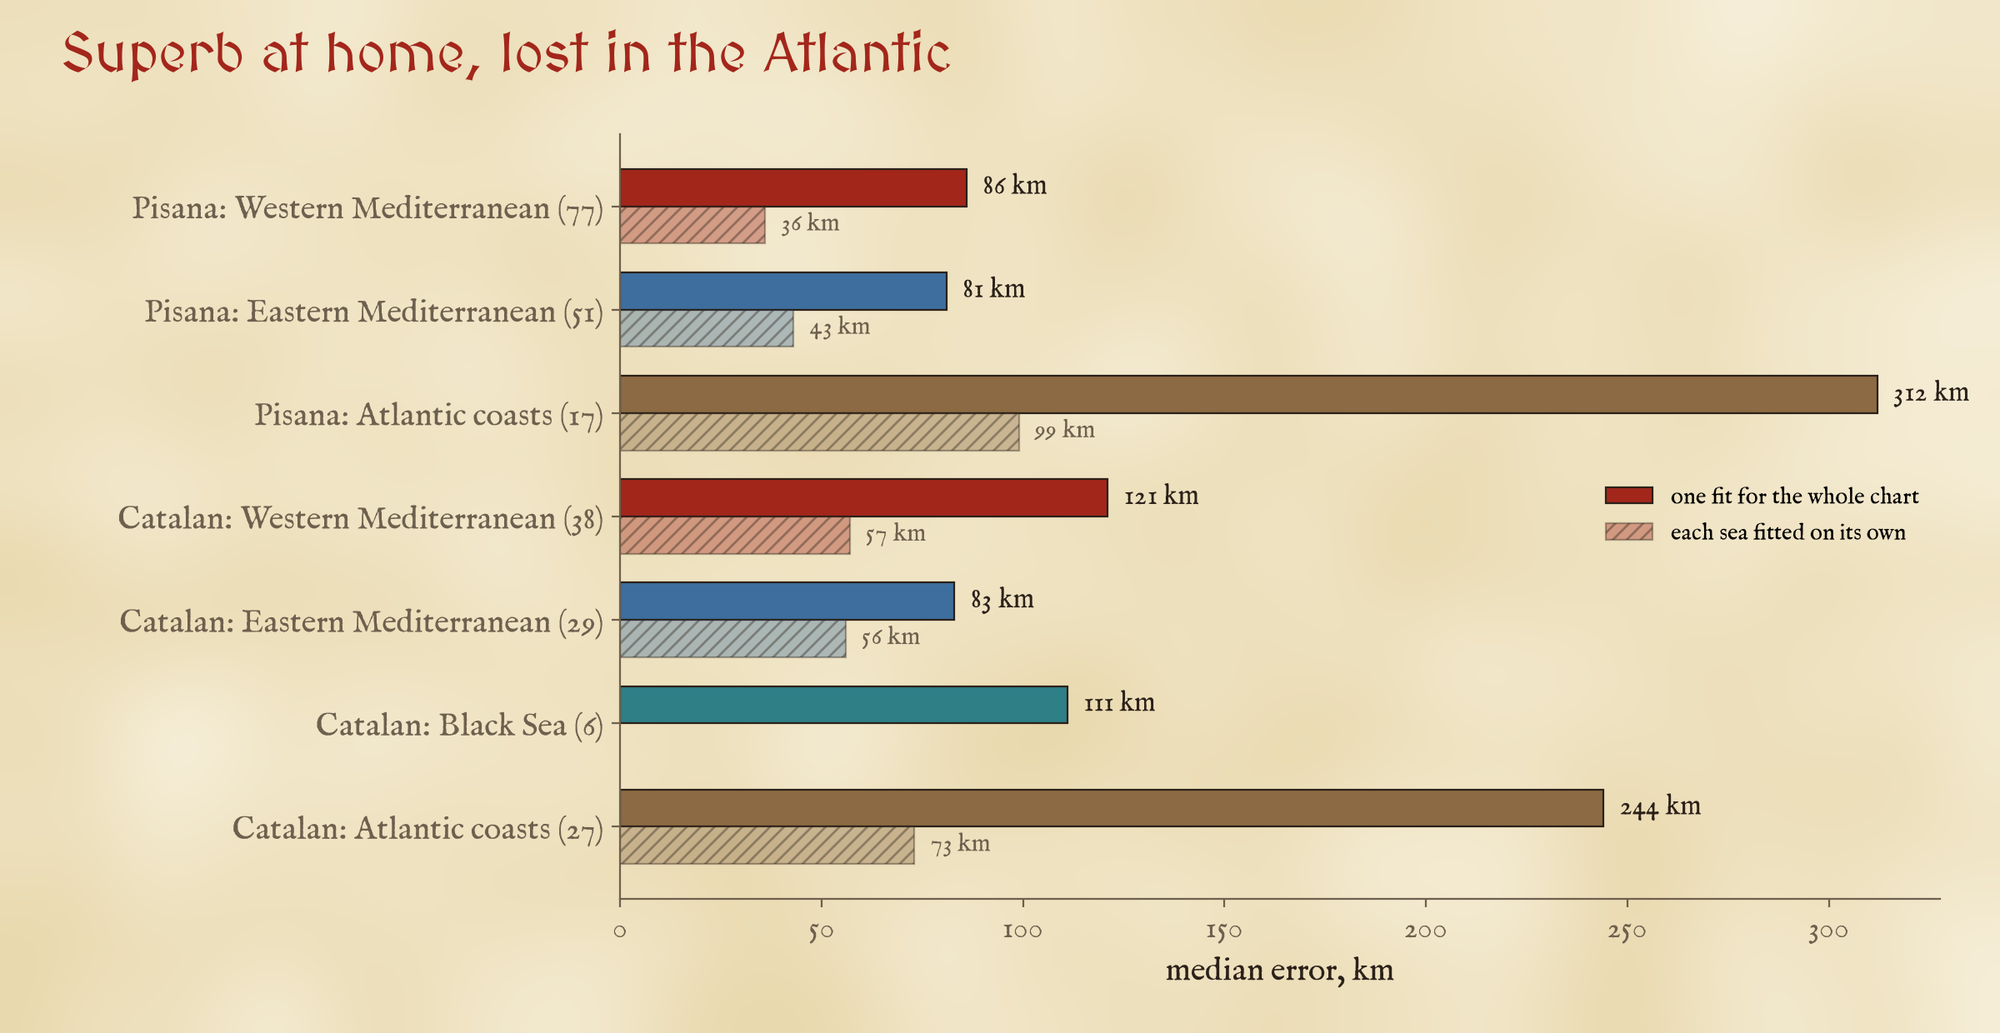
\includegraphics[width=\textwidth]{f_basins.png}
\caption{Median error by basin. Solid: one similarity fit for the whole chart. Hatched: each basin fitted on its own (basins with at least eight places).}\label{fig:basins}\end{figure}

\begin{figure}[tbp]\centering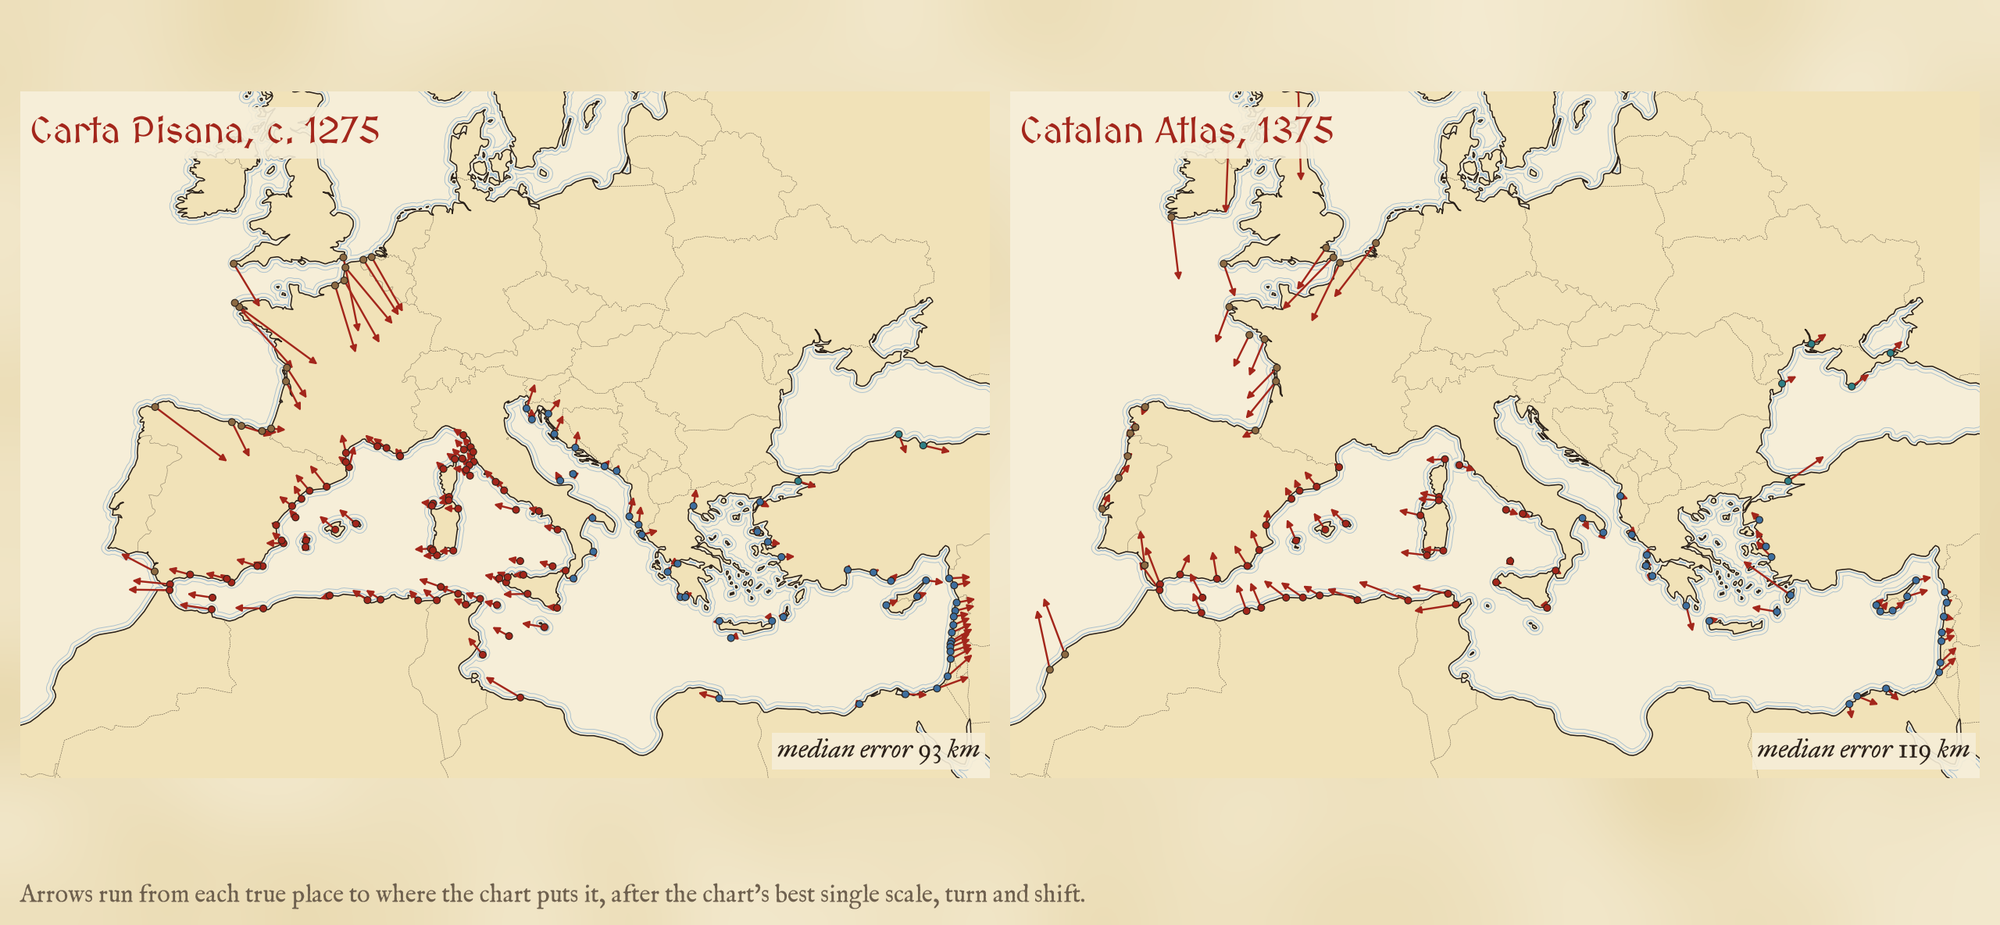
\includegraphics[width=\textwidth]{f_arrows.png}
\caption{Residuals of the whole-chart similarity fit: arrows from each true place to where the chart puts it.}\label{fig:arrows}\end{figure}

\subsection{Projection}
Table~\ref{tab:proj} and Figure~\ref{fig:proj} compare frames. For both charts the equirectangular frame fits at least as well as Mercator (86 against 93 km on the Pisana; 99 against 119 km on the Catalan Atlas), and a local azimuthal frame fits worse. With a sea that spans little more than 15 degrees of latitude the projections differ by tens of kilometres at most, comparable to the reading error, so these results do not support a Mercator-like construction but cannot rule one out \citep{nicolai2016}.

\begin{table}[tbp]\centering\small\caption{Fits in three projections: median and 90th percentile error (km) and rotation (degrees) of the similarity fit, and median and 90th percentile error of the affine fit.}\label{tab:proj}\begin{tabular}{llrrrrr}\toprule Chart & Projection & Median & P90 & Turn & Affine median & Affine P90\\\midrule
Carta Pisana & Mercator & 93 & 191 & 10.4 & 92 & 174\\
Carta Pisana & Equirectangular, 38\textdegree{} N & 86 & 179 & 10.2 & 81 & 163\\
Carta Pisana & Azimuthal equidistant & 96 & 208 & 8.8 & 107 & 204\\
Catalan Atlas & Mercator & 119 & 302 & 11.2 & 96 & 241\\
Catalan Atlas & Equirectangular, 38\textdegree{} N & 99 & 266 & 10.7 & 91 & 201\\
Catalan Atlas & Azimuthal equidistant & 134 & 302 & 9.8 & 137 & 279\\
\bottomrule\end{tabular}\end{table}

\begin{figure}[tbp]\centering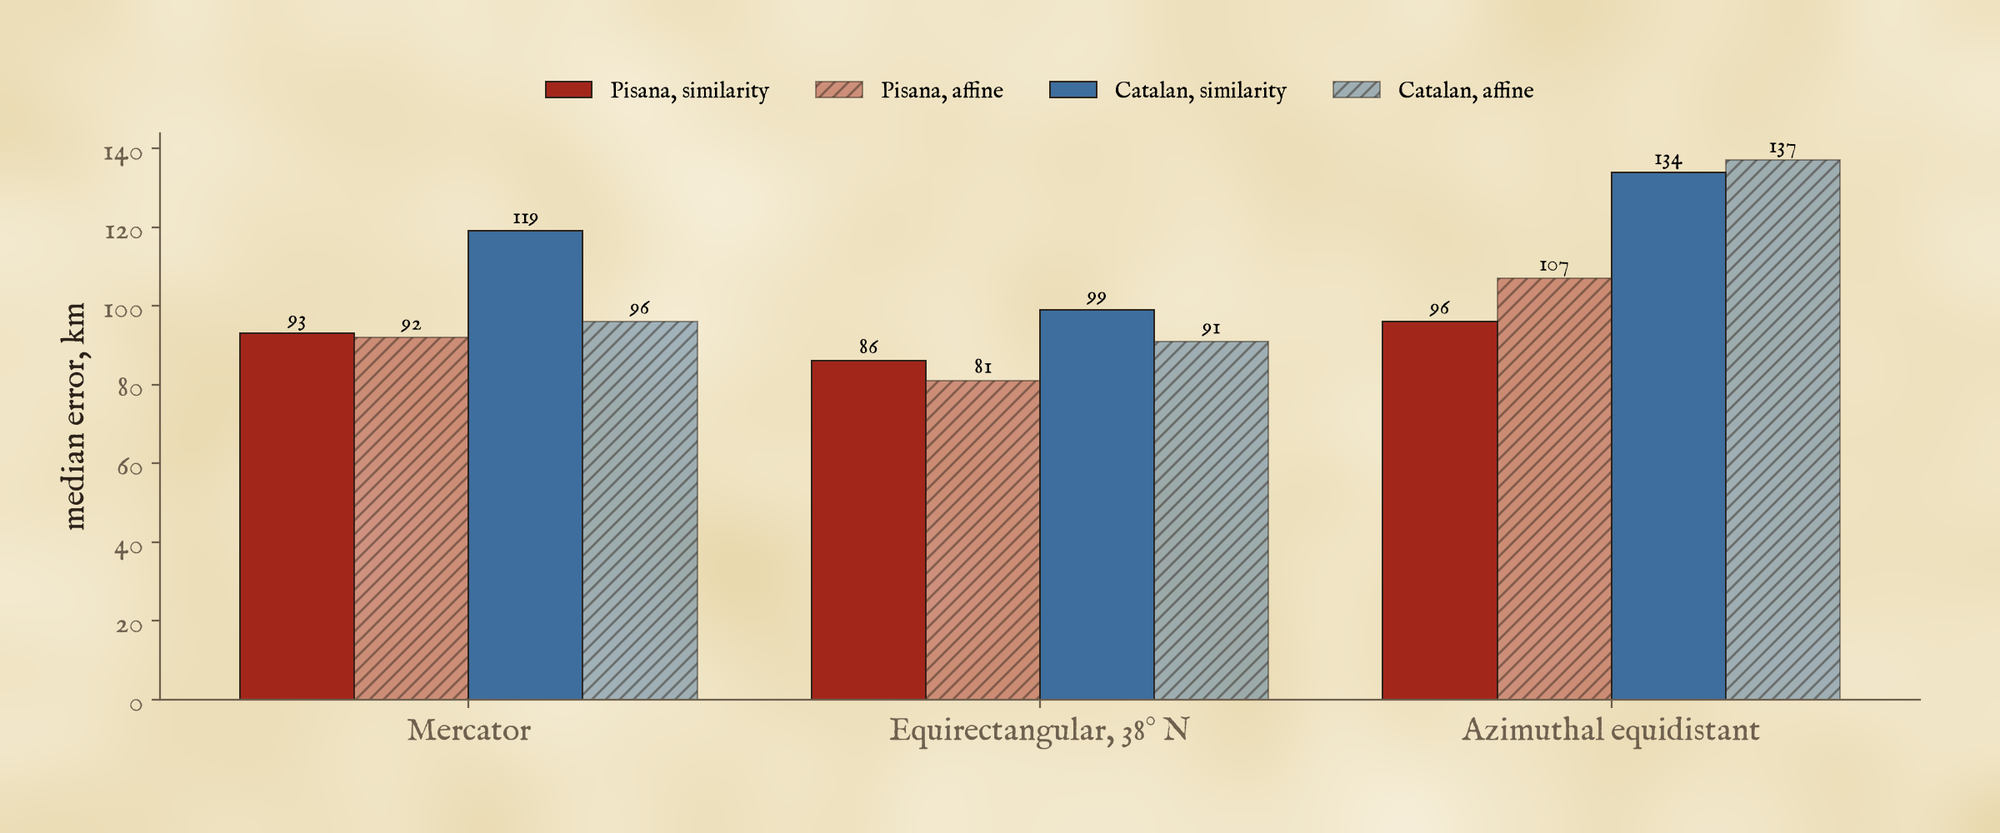
\includegraphics[width=\textwidth]{f_projections.png}
\caption{Median error of similarity and affine fits in three projections.}\label{fig:proj}\end{figure}

\subsection{Against Ptolemy, al-Idrisi and Hereford}
Figure~\ref{fig:compare} sets the two charts beside my earlier studies. Ptolemy's coordinates miss by a median 144 km after a similarity fit, over a much larger world; his regional maps of Italy and Greece, fitted on their own, miss by 74 and 52 km, against 36 and 43 km for the Pisana's two Mediterranean basins \citep{hotham_ptolemy}. Al-Idrisi's map of 1154 has a median affine error of 239 km and a local error of 55 km (44 km around the Mediterranean) \citep{hotham_idrisi}. The Hereford Mappa Mundi, contemporary with the Pisana, misses by a median 516 km \citep{hotham_hereford}. The measures differ in detail (number and spread of places, fit type), but the ranking is clear.

\begin{figure}[tbp]\centering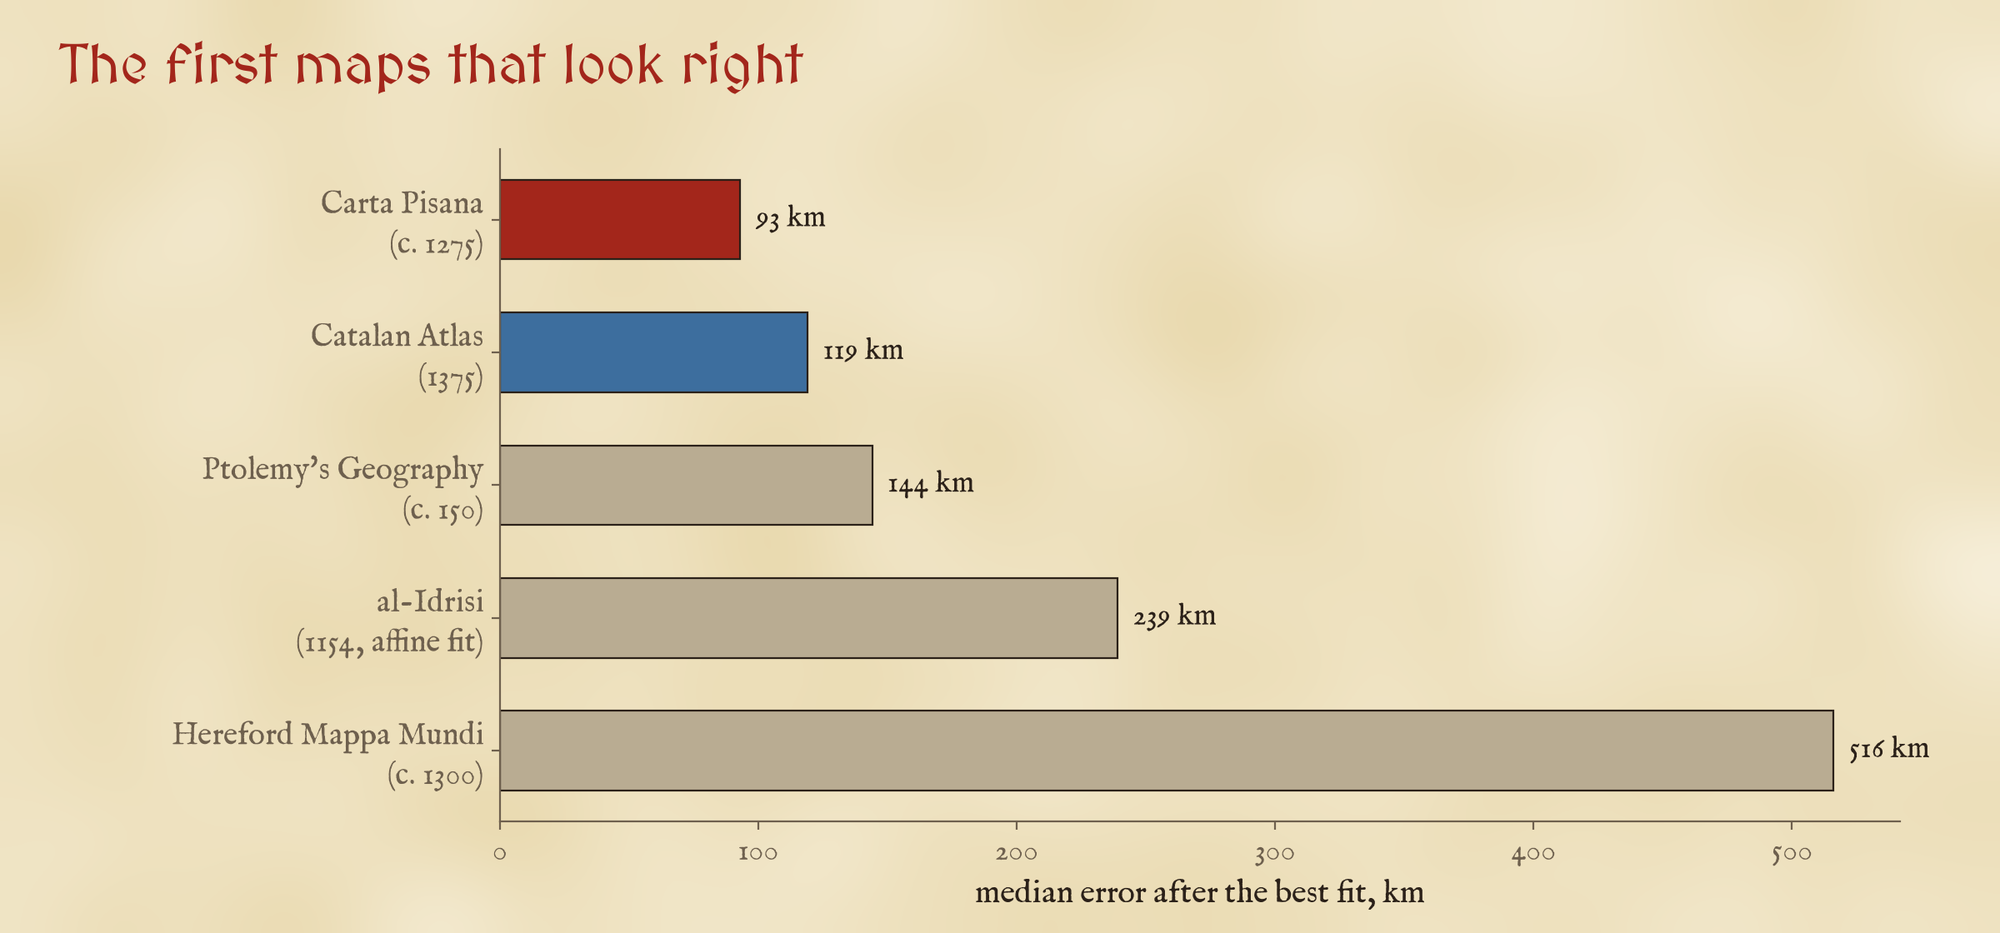
\includegraphics[width=0.9\textwidth]{f_compare.png}
\caption{Median error after the best fit: the two portolan charts against my studies of Ptolemy's Geography (similarity fit), al-Idrisi's map (affine fit) and the Hereford Mappa Mundi.}\label{fig:compare}\end{figure}

\section{Discussion}
The pattern is what a chart compiled from sailing practice would produce. The Mediterranean was sailed constantly, and the written sailing directions of the period give courses by compass wind and distances between successive harbours. A chart assembled from many such courses would be locally coherent everywhere, slightly inconsistent in scale and rotation from basin to basin, and rotated as a whole if the courses were magnetic. The Atlantic coasts beyond Gibraltar, sailed less by the same communities and with stronger tides and longer open crossings, are fitted on at the edges, smaller and misplaced; Britain on the Pisana is a schematic block. The Catalan Atlas, a century later, has better Atlantic shapes but the same displacement.

\section{Limitations}\label{sec:limits}
The control points are those I could read and identify: they favour large harbours and clear headlands and are thin in the Black Sea (only 3 on the Pisana) and on the Pisana's Atlantic coasts. Readings and identifications are mine and unreviewed; 86 Pisana and 71 Catalan readings carry the lowest confidence. The Pisana transfer adds about 37 km of noise to the facsimile readings. The scans are reproductions, and the Catalan scans are at half size; parchment shrinkage, the folds and the joining of the panels all add error. The comparison with other maps uses different numbers and kinds of places.

\section{Conclusion}
Measured on open scans, the two most famous early portolan charts place Mediterranean harbours to within a few dozen kilometres of their neighbours, get directions right to within two to four degrees once a rotation of about ten degrees is removed, and fall apart beyond Gibraltar. They are by a wide margin the most accurate maps of their age that I have measured.

\section*{Data and code availability}
The interactive page is at \url{https://maps.tristanhotham.com/portolan-charts/}. Readings, derived data and code are at \url{https://github.com/Tristan-Hotham/portolan-charts} and archived with this paper at https://doi.org/10.5281/zenodo.24044645. Readings, text and figures are CC BY 4.0 and code MIT; the chart scans are public domain.

\section*{AI statement}
I wrote the text, with drafting and editing assistance from Claude (Anthropic), which also helped prepare the analysis code. I reviewed and checked all text and results.

\begin{thebibliography}{9}
\bibitem[Campbell(1987)]{campbell1987} Campbell, T. (1987) Portolan charts from the late thirteenth century to 1500. In Harley, J. B. and Woodward, D. (eds) \textit{The History of Cartography, Volume One}. Chicago: University of Chicago Press, 371 to 463.
\bibitem[Hotham(2026a)]{hotham_hereford} Hotham, T. (2026a) The world according to the Hereford Mappa Mundi: a medieval map of the world set against a modern one. Zenodo. \url{https://doi.org/10.5281/zenodo.23878612}
\bibitem[Hotham(2026b)]{hotham_idrisi} Hotham, T. (2026b) Al-Idrisi's World: the map made for Roger II of Sicily in 1154, set against a modern map. Zenodo. \url{https://doi.org/10.5281/zenodo.23882607}
\bibitem[Hotham(2026c)]{hotham_ptolemy} Hotham, T. (2026c) Ptolemy's world, measured: the coordinates of the Geography set against a modern map. Zenodo. \url{https://doi.org/10.5281/zenodo.23882603}
\bibitem[Jomard(1842)]{jomard} Jomard, E. F. (1842 to 1862) \textit{Les monuments de la g\'eographie}. Paris.
\bibitem[Lanman(1987)]{lanman1987} Lanman, J. T. (1987) \textit{On the Origin of Portolan Charts}. Chicago: The Newberry Library.
\bibitem[Natural Earth(2026)]{ne} Natural Earth (2026) Land and admin 0 countries. Public domain. \url{https://www.naturalearthdata.com/}
\bibitem[Nicolai(2016)]{nicolai2016} Nicolai, R. (2016) \textit{The Enigma of the Origin of Portolan Charts: A Geodetic Analysis of the Hypothesis of a Medieval Origin}. Leiden: Brill.
\bibitem[Pujades(2007)]{pujades2007} Pujades i Bataller, R. J. (2007) \textit{Les cartes portolanes: la representaci\'o medieval d'una mar solcada}. Barcelona: Institut Cartogr\`afic de Catalunya.
\end{thebibliography}
\end{document}
